
%%%%%%%%%%%%%%%%%%%%%%%%%%%%%%%%%%%%
%						Deep Neural Network 
%
%	 Author: Valgi0
%
%  Goal: All notes from various sources 
% 
%%%%%%%%%%%%%

\documentclass[12pt,a4paper,twoside,openright]{scrbook}

\usepackage[utf8]{inputenc}
\usepackage[english]{babel}
\usepackage[T1]{fontenc}


\usepackage{amsmath,amsfonts,amssymb,amsthm}
\usepackage{caption}
\usepackage[usenames]{color}
\usepackage{enumerate}
\usepackage{fancyhdr}
\usepackage{fancyvrb}
\usepackage{float}
\usepackage{graphicx}
\usepackage{booktabs}
\usepackage{indentfirst}
\usepackage{listings}
\usepackage{marvosym}
\usepackage{multicol}
\usepackage{sectsty}
\usepackage{subcaption}
\usepackage{tocloft}
\usepackage{microtype}
\usepackage[table]{xcolor}
\usepackage{url}
\usepackage{hyperref}
\usepackage{adjustbox}
\usepackage{blindtext}


\hypersetup{%
	pdfpagemode={UseOutlines},
	bookmarksopen,
	pdfstartview={FitH},
	colorlinks,
	linkcolor={black},
	citecolor={black},
	urlcolor={black}
}


\makeindex

\subject{my note about}
\title{Basic (and Maybe advanced) Deep Learning stuff }
\subtitle{theory and samples}
\author{Valgi0 (me as always)}

\begin{document}

\frontmatter 

\maketitle


\newpage

\tableofcontents

\newpage

\listoffigures

\mainmatter

\pagestyle{fancy} 
\fancyhead[LO]{\nouppercase{\rightmark}}
\fancyhead[RE]{\nouppercase{\leftmark}}
\fancyhead[LE,RO]{\thepage}
\fancyfoot{}

%% CAPITOLO 1
\chapter{Why this documents}
I feel the exigence to put together all my notes and my experience in this wide word of Deep Neural Network. I want them in one place with a good organization allowing me and the reader to access to what I need quickly. This thought came to my mind while I was working to my dissertation thesis, and for the haste, I used to write notes every where and when I needed them they were hard to find. Btw I don't care to write why I'm doing this so

\section{Where Information come from}
I'm going to use some books freely distributed and one day I'll put the links here. Stay tuned

\section{Chapters organization}
Each chapter contains arguments to one topic and information are organized following this schema:
\begin{itemize}
\item Introduction to the topic
\item Theory about topic
\item Examples maybe
\item Related links or papers ( Idk )
\end{itemize}

\section{Notation}
\begin{itemize}
\item \textit{a,b,c} are scalars
\item \textbf{a,b,c} are vectors
\item \textbf{A,B,C} are matrices
\item \textbf{0} it is a zero vector
\end{itemize}

\chapter{Has someone said Math?}

In this chapter we are going to explore all math stuff we need to fully understand the concepts.
If God Exists he must be a mathematician.

\section{Linear Algebra OMG}

Let's start by defining what is a vector.. a vector is a vector. $\textbf{v} = [i_0, i_1, i_2, ... , i_n]$. In this case $v$ is a vector composed by elements $i \in \mathbb{I}$ with size $n$. So vector comes from $\mathbb{R}^n$ space. This is the n-dimensional Euclidean Space. A vector with all zeros is called \textbf{zero vector} and it will be represented as $\textbf{0}$

\subsection{Vector Space}
The Vector Space $\mathbb{X}$ is a set of vectors that satisfies the following conditions:
\begin{itemize}
\item \textbf{Addition Closure}. This means that:
\begin{itemize}
 \item if $\textbf{x}, \textbf{y} \in \mathbb{X}$ so $\textbf{x} + \textbf{y} = \textbf{j}$ and $\textbf{j} \in \mathbb{X}$ for each $\textbf{x,y}$
 \item  $\textbf{x} + \textbf{y} = \textbf{y} + \textbf{x}$
 \item  $\textbf{x} + (\textbf{y} + \textbf{c}) = (\textbf{x} + \textbf{y}) + \textbf{c}$
 \item $\textbf{x} + \textbf{0} = \textbf{x}$
 \item For each $x \in \mathbb{X}$ exists a unique vector called $\textbf{-x}$ such that $\textbf{x} + (\textbf{-x}) = \textbf{0}$
 \end{itemize} 
\item \textbf{Multiplication Closure}. This means that if $\textbf{x} \in \mathbb{X}$ and $y$ a scalar so $\textbf{x} * y = \textbf{j}$ and $\textbf{j} \in \mathbb{X}$ for each $\textbf{x,y}$ \begin{itemize}
\item $\textbf{x} * 1 = \textbf{x}$
\item For any $a, b$ scalars $(ab)*\textbf{x} = a(b*\textbf{x})$
\item $(a + b)*\textbf{x} = a*\textbf{x} + b*\textbf{x}$
\item $a(\textbf{x} + \textbf{y}) = a*\textbf{x} + a*\textbf{y}$
\end{itemize}
\end{itemize}

From the above conditions we can extract some considerations. The first is that each $\mathbb{R}^n$ is a vector space. A subset of this euclidean space can be a vector space only if it his unbounded. For example:
\newline
\[ \mathbb{X} = ( (x,y) : x < 5  y < 5, (x,y) \in \mathbb{R}^2)\] \newline \[
v_0 = (4,4), v_1 = (3,3) \in \mathbb{X}\] \newline \[
v_0 + v_1 = v_2 = (7,7) not \in \mathbb{X}
\]
So $\mathbb{X}$ is not a vector space.

\subsection{Linear Independence}
\textbf{Linear combination} is a very cool stuff. Let's have a vector $\textbf{x}$ and some different vectors $\textbf{y,z,k}$. If there exists a set of three scalars such that $a_0*\textbf{y} + a_1*\textbf{z} + a_2*\textbf{k} = \textbf{x}$ so $a_0*\textbf{y} + a_1*\textbf{z} + a_2*\textbf{k}$ is a linear combination.
Linear indipendence is a propery between more vectors. $\textbf{x}_0, \textbf{x}_1,...,  \textbf{x}_n$ are linearly dependent  just if there exist $n$ scalars at least one of which is not zero, that:
\[a_0\textbf{x}_0 + a_1\textbf{x}_1 +  ... + a_n\textbf{x}_n = \textbf{0} \]
Otherwise, if all $a_i$ are 0, vectors are \textit{linearly independent}.
\textbf{Attention} if a set of vectors is linearly dependent so one or more that tis vectors can be obtained by a linear combination of others.
\newline
\textbf{Let's do some examples}
\[\textbf{v}_0 = [1,-1], \textbf{v}_1=[-1,1] , \textbf{v}_2 = [-1,-1]\]
These are three vectors. Are they linearly independent?
\[a_0*\textbf{v}_0  +  a_1*\textbf{v}_1 + \textbf{v}_2*a_2  = 0 \rightarrow \begin{bmatrix}
 a_0 - a_1 - a_2 = 0 \\ -a_0 + a_1 - a_2 = 0
\end{bmatrix} \]
Now we need to solve those equations:
\[a_0 = a_1, a_2 = 0\]
So they are a linear dependent vectors. This means that we can select one of them and express it as a linear combination of the others:
\[\textbf{v}_0 = \textbf{v}_1*a_1 + \textbf{v}_2*a_2\]
That is true for $a_1 = -1$ and $a_2 = 0$.

\subsection{Spanning a Vectors space}
To create a vector space we can grab some vectors and create this space as the set of all linear combinations of these vectors. It the given vectors are linearly independent they are called \textbf{Basis set} for that vector space. The number of vectors in the basis set is the dimension of the vector space. This means that we can express each vector inside that space using a number of independent vectors equal to the dimension of the space.\newline
\textbf{For Example} $\mathbb{R}^2$ can have as basis $(1,0), (0,1)$. Using these two vectors we can create each vector inside the space. Try to believe.

A vector space can have infinite basis. But the basis composed by binary vectors

\subsection{Some functions}
Some functions can be defined between vectors. the first is the \textbf{Inner Product} that is the product between two vector and it is represented with $(\textbf{x}, \textbf{y})$. This function must follow these properties:
\begin{itemize}
\item $(\textbf{x}, \textbf{y}) = (\textbf{y}, \textbf{x})$ 
\item $\textbf{x} (a \textbf{y} + b \textbf{j}) = a(\textbf{x}, \textbf{y}) + b(\textbf{x}, \textbf{j})$
\item $(\textbf{x}, \textbf{y}) \geq 0$ if $\textbf{x}$ is not the zero vector.
\end{itemize}
The standard inner product adopted the respect the above properties is:
\begin{equation}
\textbf{x}\textbf{y} = x_{0}y_{0} + x_{1}y_{1} + ... + x_{n}y_{n}
\end{equation}

Another function that can be defined is the \textbf{Norm} represented by $\parallel \textbf{x} \parallel$. This function must respect these properties:
\begin{itemize}
\item $\parallel \textbf{x} \parallel \geq 0$
\item $\parallel \textbf{x} \parallel = 0$ if $\textbf{x}$ is the zero vector
\item $\parallel a\textbf{x} \parallel = \mid a \mid \parallel \textbf{x} \parallel$
\item $\parallel \textbf{x} + \textbf{y} \parallel \leq \parallel \textbf{x} \parallel + \parallel \textbf{y} \parallel$
\end{itemize}
There are many function that satisfy these conditions. The most common \textbf{norm} is:
\begin{equation}
\parallel \textbf{x} \parallel = (\textbf{x}\textbf{x})^{\frac{1}{2}} = \sqrt{x_0^2 + x_1^2 + ... + x_n^2}
\end{equation}

Using both of the previous function we can define the \textit{angle} between two vectors. In particular we can calculate the \textit{cosine}:
\begin{equation}
cosine(\textbf{x},\textbf{y}) = \frac{ \textbf{x}\textbf{y}}{\parallel \textbf{x} \parallel \parallel \textbf{y} \parallel}
\end{equation}
 
 \section{Linear Transformation}
 For \textbf{Transformation} we identify the operation that relate a value x to a value y. Let's define:
 \begin{itemize}
 \item \textit{Domain} the set of $x_i \in \mathbb{X}$ values.
 \item \textit{Range} or Co-domain the set of $y_i \in \mathbb{Y}$ values
 \item \textit{Transformation} as the rule relating each $x_i$ to an $y_i$ 
 \end{itemize}
 
 A transformation $A$ is \textit{Linear} if:
 \begin{itemize}
 \item for all $x_0, x_1$ $A(x_0 + x_1) = A(x_0) + A(x_1)$
 \item for all $x_0$ and for all $a$ scalars $A(x_0*a) = A(x_0) * a$   
 \end{itemize}
 
 \textbf{IMPORTANT}\\
 \emph{For any transformation between two finite dimensions vector space can be represented by a Matrix. This Matrix is build using the basis of the vector spaces so changing them the matrix change}
 
 \subsection{Eigenvalues eigenvectors}
 All vectors from a Vector space not $0$ and scalars that make this equation true:
 \begin{equation}
 A(\textbf(z)) = a\textbf(z)
\end{equation}  
are called Eigenvalues and eigenvectors. 
What that means?? Graphically the eingenvector of a Linear transformation is the direction for which vectors in that direction that after the transformation will have the same direction but a different length.

\subsubsection{How to compute them}
In order to compute them let's  take a look to the formula:
\[ A(\textbf{z}) = a\textbf{z} \]
We said that a linear transformation can be represented by a matrix so the formula becomes:
 \[ \textbf{A}\textbf{z} = a\textbf{z} \]
 \[(\textbf{A} - a\textbf{I}) * \textbf{z} = 0\]
 Let's define \textbf{A} matrix as:
 \[\begin{vmatrix}
-1 & 1\\0 & -2 
 \end{vmatrix}\]
 so $(\textbf{A} - a\textbf{I}) = 0$ (Now we look for determinant that is 0,.. dont ask why) is:
  \[\begin{vmatrix}
-1 - a & 1\\0 & -2 - a
 \end{vmatrix} = 0 \]
The solutions are found solving:
\[a^2 + 3a + 2 = (a + 1)(a + 2) = 0 \Rightarrow a_0 = -1 a_1=-2\]
Those are the eigenvalues. To find the vectors you must solve the equation \[(\textbf{A} - a\textbf{I}) * \textbf{z} = 0\] using each eigenvalue.
\chapter{Let's start}

In this chapter we are going to see the very basic of Neural Network like \textit{Neurons}, \textit{Links}, \ldots.

\section{Single Neuron}
Neuron is the basic unit of Neural Network and is just a mathematical function applied to an input.
Let's define an input a scalar \textit{i} a scalar weight \textit{w}, a scalar bias \textit{b} and a function \textit{f}.
Neuron function is:
\begin{equation}
a = f(iw + b)
\end{equation}
Function \textit{f} is called \textbf{Activation Function} or sometimes \textbf{Transfer function} and usually is a non linear function.

\subsection{Example of neuron}
\textit{i} = 5, \textit{w} = 0.5, \textit{b} = 2 and \textit{f(x)} = $x + 1$  
\begin{equation}
f(5*0.5 + 2) = f(4,5) = 5.5
\end{equation}

\section{Transfer functions}
\begin{figure}
    \centering
    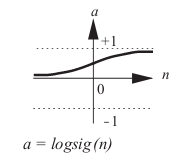
\includegraphics[scale=0.65]{img/log-sigmoid-function.png}
    \caption{log-sigmoid function}
    \label{img:log-sigmoid}
\end{figure}{}
Or Activation function are chosen during model creation in fact they are Hyper-Parameters. They can be linear or non-linear. Now some of the most important linear functions are listed:
\begin{itemize}
\item \textbf{Hard Limit Transfer Function}. This function produce 0 if input value is negative or 1 if value is equal or greater that 0. It creates a step and it is used for binary classification problems
\item \textbf{Linear Function}. $f(x) = x*m +q$. It is the function of the line.
\item \textbf{log-sigmoid transfer function}. $f(x) = \frac{1}{1+e^{-x}}$. This function produce a value always positive and you can see the graphic at the figure \ref{img:log-sigmoid}
\end{itemize}
\begin{figure}
    \centering
    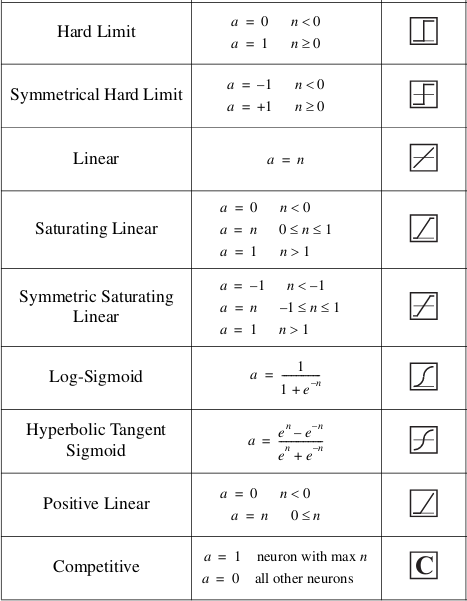
\includegraphics[scale=0.65]{img/activation-functions-table.png}
    \caption{Overview of basic activation functions}
    \label{img:activation-functions-basic}
\end{figure}

\subsubsection{Diagonalization}

A matrix that represents a linear transformation can be \textit{Diagonilized} by changing the basis in the one composed with only Eigenvectors. Each dimension is represented by one of those vectors so the matrix has to contain all eigenvalues to perform such operation. In this way it become a diagonal matrix filled by eigenvalues. 

\section{Multi-input Neuron}
Usually neuron has more than one input at time. Each of them want a private \textit{w} while \textit{b} the bias is one for all. Under this light we can say that input \textbf{i} is a column vector of $i_0,.., i_n$ elements and neuron contains a scalar \textit{b} and a vectors of \textbf{w} of n weights. Using \textit{f} as linear function $f(x) =x + 1$ the neuron perform this equation:
\begin{equation}
a = f(\textbf{wi} + b) = f((\sum_{j=0}^{n} w_j * i_j) + b)
\end{equation}

\subsection{Example}
\textbf{i} = $5,6,7$ \textbf{w} = $1,2,-1$ \textit{b} = 2 and \textit{f(x)} = $x + 1$  
\begin{equation}
f(5*1 + 6*2 + 7*-1 + 2) = f(12) = 13
\end{equation}

\section{Multi-neurons}
Often Input vector goes to multiple neurons and these neurons are a Layer. It is important keep in mind that:
\begin{itemize}
\item All Neurons take all input. So \textit{w} weights is a vector with the same dimension of the input vector
\item All Neuron produce a scalar so the number of neurons in a layer is the number of  outputs.
\item Each neuron has its bias so a layer has a vector of bias one per neurons 
\end{itemize}

Let's define input \textbf{i} a column vector and weight \textbf{W} as a matrix $m*n$ where $m$ is the number of the neuron and $n$ the number of the input elements in \textbf{i}. \textit{f} is the activation function:

\begin{equation}
\textbf{a} = f(\textbf{W}\textbf{i} + b)
\end{equation}

From the above equation we can see that a matmul is performed between weights matrix and input column vector. So row $j$, that is the weight vector of the neuron $j$ is multiplied and summed with the whole input column vector.

\begin{equation}
  \begin{bmatrix}
w_{0,0} & w_{0,1} & \ldots & w_{0,n} \\
w_{1,0} & w_{1,0} & \ldots & w_{1,n} \\
\vdots & \vdots & \vdots & \vdots \\
w_{m,0} & w_{m,1} & \ldots & w_{m,n} \\
  \end{bmatrix} * \begin{bmatrix}
  i_0 \\ i_1 \\ \vdots \\ i_n
  \end{bmatrix}
\end{equation}

So a neural layer can be seen as a matrix of weight and a Bias vector:
\begin{equation}
Layer_w = \begin{bmatrix}
n_0 \\ n_1\\ n_2\\ \vdots \\ n_m
\end{bmatrix} = \begin{bmatrix}
w_{0,0} & w_{0,1} & \ldots & w_{0,n} \\
w_{1,0} & w_{1,0} & \ldots & w_{1,n} \\
\vdots & \vdots & \vdots & \vdots \\
w_{m,0} & w_{m,1} & \ldots & w_{m,n} \\
\end{bmatrix}
\end{equation}
\begin{equation}
Layer_b = [b_0, b_1, b_2, \ldots , b_m]
\end{equation}

Mathematically a layer can be represents just by \textbf{W} the weight matrix and \textbf{b} the bias vector.

\section{Multi Layers}

A neural network has more layers. The first layer is called \textbf{Input layer} the last in called \textbf{Output layer} and the ones in the middle are \textbf{Hidden Layers}. 
Each layers can have different number of neurons and different activation function. So a basic multi-layer network with $l$ layers is defined by $f_0, ..., f_l$ activation functions, $\textbf{W}_0,..., \textbf{W}_l$ weight matrices and $\textbf{b}_0,...,\textbf{b}_l$ or just \textbf{B} bias (matrix contains in row $j$ the bias vector for the layer $j$).
This network take inputs with the first layer, generate output and then gives this output to the second layer and so on.
A Multi layer Network performs:
\begin{equation}
\textbf{a} = f_l(f_{l-1}(\ldots * \textbf{W}_{l-1} + \textbf{b}_{l-1}) * \textbf{W}_{l} + \textbf{b}_{l})
\end{equation}

This Multi-layer neural Network is called \textbf{Feed Forward Neural Network}

\section{Recurrent Neural Network}
Feed forward neural network has layers and layer has neurons. Each Neuron take a input vector \textbf{i} and produce a scalar \textit{a}. Differently, Recurrent Neural Network takes two input vector the input vector \textbf{i} and some \textit{a'} that is the output of the previous input. Let's imagine we have a time series of data $i_0,...,i_t$. This data must be given to the model respecting the sequence but we want model somehow remember previous data. For this kind of task Recurrent Neural Network was created. They have layers and neurons but each neuron has two vectors and a bias: \textit{u} weights for the input, \textit{w} weights for its layer output at the previous step and \textit{b} the bias. Let me explain in a intuitive way before using math: the input is a series of vectors. First vector $i_0$ is taken and is given to the first layer of the model. Each neurons of this layer get the input vector $i_0$ and produce a scalar $a_0$ and with other neurons output of that layer it creates the layer output \textit{a}  Nothing new until now. Output goes to the second layer and so on until last layer. Second input is taken $i_1$ and neuron  receives it and the previous layer output \textit{a}. Using both of them it compute the next scalar output $nexta_0$. And so on! 

Let's define its behavior using some cool math. Our network is composed by 1 layer with 1 neuron:
\begin{equation}
  inputsequence= \textbf{i}_0, \ldots ,\textbf{i}_k 
\end{equation}
\begin{equation}
  f_{neuron} = ActivationFunc( b + \textbf{w}*a'_{t - 1} + \textbf{u}*\textbf{i}_t) = a_{t}
\end{equation}
The neuron takes at time t in input $a'_{0,t - 1}$ and $i_{0,t}$ and produce $a_{t}$. In this case with just one neuron the layer output coincide with the neuron output. After that the following equation is performed to compute $a'_t$
\begin{equation}
a'_t = c + \textbf{v}a_t
\end{equation}

Let's imagine to have a Recurrent Neural Network with more layers and more neurons for each layers. The above equations become:
\begin{equation}
\textbf{a}_t = ActivationFunc(\textbf{b} + \textbf{W}*\textbf{a'}_{l,t-1} + \textbf{U}*\textbf{i}_t)
\end{equation}
$a'_{l,t-1}$ means the column vector output from the layer $l$ at time step $t-1$
\begin{equation}
\textbf{a'}_{l,t} = \textbf{c} + \textbf{V}\textbf{a}_{l,t} 
\end{equation} 

That is all my dear.. Not true, we are going to expand this kind of network later

\subsection{Keep in mind}
Some tips to keep in mind when you work with Recurrent Neural Network
\begin{itemize}
\item Externally are similar to feed forward network.. it has layers and neurons
\item The inputs are sequence of inputs vectors
\item Output is a series of vectors one for each inputs vector but if a prediction is what u want last output must be used.
\item At any time neuron takes exactly 2 input vectors in input and they are the output from prior layer and output for its layer but a time t-1. 
\item For each input vectors neurons has a weight vector this means that a layer has a \textbf{W} and \textbf{U} weight. The first for its own output and the second for the output of the previous layer.
\item Output of a layer is turned in a input performing $c + \textbf{V}a_l$ where c is a bias and \textbf{V} is a weight matrix.
\end{itemize}

\section{Some Applications}
In this section we are going to see how the previously explained network are used in a very easy problem:
\emph{
We have some fruits composed by oranges and apples and we need a model capable to tell us if a given fruit is one or it is the other. Fruits is defined by size, dimension, weight.
}

Let be $i_a = \begin{vmatrix}
1 & -1 & -1
\end{vmatrix}$ the vector that represent an apple and  $i_o = \begin{vmatrix}
1 & 1 & -1
\end{vmatrix}$ the one that represent an orange. 

\subsection{Perceptron}
Perceptron is a binary classifier based on single layer \textbf{Feed Forward Network} with \textbf{Hard Limit} as activation function. So if the output is minor than 0 the function produces 0 otherwise 1.

\begin{equation}
output = HardLims(\textbf{W}\textbf{i} + \textbf{b})
\end{equation}

\textbf{W} is a matrix $nxm$ where n is the dimension of the input vector (3 in this case) and $m$ the number of neurons in the layer.

Let's define $W = [0, 1, 0]$ for a single neuron layer. This is called \textbf{Single-Neuron Perceptron}. Now we can test it against our data.
\newline
\textbf{Apple} defined as  $i_a = \begin{vmatrix}
1 & -1 & -1
\end{vmatrix}$ is multiplied by \textbf{W}
\begin{equation}
[0, 1, 0] * \begin{vmatrix}
1 & -1 & -1
\end{vmatrix}^T = 0*1 + 1*-1 * 0*1 = -1
\end{equation}
\textit{For simplicity input vector is not in column but it should be. Don't judge me}
\begin{equation}
hardlims(-1) = -1
\end{equation}
Ok! model classify apple as -1 let's check if orange are classified as 1
\begin{equation}
[0, 1, 0] * \begin{vmatrix}
1 & 1 & -1
\end{vmatrix}^T = 0*1 + 1*1 * 0*1 = 1
\end{equation}
\begin{equation}
hardlims(1) = 1
\end{equation}

OMG!!!! That is amazing... or not but anyway with a weight vector $[0, 1, 0]$ model is able to classify the fruits. Now try with banana and tell me if it works! COME ON!

\chapter{Basic Concepts about learning rules}
In this chapter we are going to study in deep the basic concepts about learning rule. With  \textit{learning rule} it means all the rules and algorithms used to modify the weight and the bias of the network in order to improve the results.
There are three main approaches:
\begin{itemize}
\item \textit{Supervised learning}. In this case the net is trained by using a set of examples composed by $(p_0, t_0)$ where $p_0$ is the input for the network and $t_0$ the corresponding correct result (target). The result produced is compared to the target. The learning rules are used to modify weights to make model produce the right result. 
\item \textit{Reinforcement Learning}. The algorithm produce a score or a grade according to the network performance and the learning rule seek to adjust weights in order to get higher scores. The network continues to learn also during its application.  
\item \textit{Unsupervised Learning}. The data does not have the target but they are somehow clustered. The cluster becomes the target to predict like the one in the supervised learning.
\end{itemize}

Probably, we will speak about all this approaches later.

\section{Learning rules for Perceptron Architecture}

\subsection{Perceptron Network again}
\begin{figure}
    \centering
    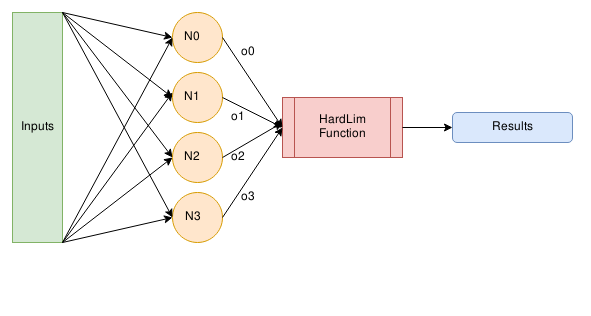
\includegraphics[scale=0.65]{img/PerceptronNetwork.png}
    \caption{Overview of a Perceptron Network}
    \label{img:perceptron_network}
\end{figure}
The perceptron network has a single layer of $S$ neurons and it use as activation function the \textbf{Hardlim} (it produce 0 or 1 according to the output of the neuron).
The weights of the network are:
\begin{equation}
\textbf{W} = \begin{bmatrix}
\textbf{w}_0 \\ \textbf{w}_1 \\ \vdots \\ \textbf{w}_s 
\end{bmatrix}
\end{equation}

So each neuron has a list of $w_{n0}, ... , w_{nm}$ weights where $n$ it the neuron and $m$ is the number of weight and it is the same for the number of inputs.

Each neuron produce a result $o_n$ and the list with all results from all neurons is given to the activation function.

\section*{the decision boundary}
Let's use a Perceptron Network with one neuron and 2 inputs. The result is obtained by this formula:
\begin{equation}
o = hardlim((w_0 * p_0 + w_1 * p_1) + b)
\end{equation}
The decision boundary of the network is determined by the sub set of inputs that make the neurons produce zeros.
\newline
\textbf{Example:}
Let's have $w_0 = 1$, $w_1= 1$ and $b = -1$. So the decision boundary will be:
\begin{equation}
(w_0 * p_0 + w_1 * p_1) + b = p_0 + p_1 - 1 = 0 \Rightarrow p_0 + p_1 = 1
\end{equation} 

The decision boundary define a line in the input space. On one side of that line, the network output will be 0, on the other side will be one.
\begin{figure}
    \centering
    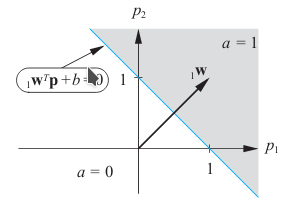
\includegraphics[scale=0.5]{img/decision_boundary_for_perceptron.png}
    \caption{Graphic representation of the decision boundary}
    \label{img:perceptron_network}
\end{figure}
Modifying the weights and the bias of the network this line is moved up and down changing also its orientation.

\subsection{Decision Boundary for Multiple Neurons}
Network with $S$ neurons has $S$ lines, one for each of them. So each neuron can classify each input in just two categories. A network with one neuron has one decision boundary so it can produce just 2 category, while a network with S neurons can produce $2^s$ different output vectors so it can be used to classify an input to these categories.

\section{Learning rules for Perceptron Network}
There is a precise algorithm that tells us how to update the weights and it guarantees the best solution is found.
The idea behind is if the model predict the wrong result weight must be modified to let the model classify that input. For this case let's define $e = t - a$ where $t$ is the target and $a$ is the output of the model. Each weight is updated according to this formula:
\begin{equation}
\textbf{w}^{new} = \textbf{w}^{old} + e\textbf{p}
\end{equation}
We can do the same for bias: Bias are just single weight for an input that is always one.
\begin{equation}
b^{new} = b^{old} + e
\end{equation}

So, the perceptron rule can be written for the matrix of weight in case the network has more than one neuron.

\begin{equation}
\textbf{W}^{new} = \textbf{W}^{old} + \textbf{e}\textbf{p}
\end{equation}
\begin{equation}
\textbf{b}^{new} = \textbf{b}^{old} + \textbf{e}
\end{equation}

\textit{That is all by now, but there is a proof of convergence that demonstrates this algorithm always find the best solution}.

\subsection{Example}
Let's have a singular-neuron perceptron network for 3-input vectors: $i_0 = [1,-1,0]$, $i_1 = [1,1,-1]$, $i_2 = [1,0,0]$. For all of them we have the corresponding targets $t_0 = 1,  t_1 = 0,  t_2 = 1$. Let's initialize our net with random values: $w = [0, 0.5, -0.2], b = 0.3$.
\newline
First, it can be useful find out the decision boundary:
\begin{equation}
(0*i_{n0} + 0.5 * i_{n1} - 0.2 * i_{n2}) + 0.3) = 0 \Rightarrow \frac{i_{n1}}{2} - \frac{i_{n2}}{5} = 0.3
\end{equation}

Now we can proceed giving the first input to the network and see what happend:
\begin{equation}
hardlim((0*1 + 0.5 * -1 - 0.2 * 0) + 0.3) = hardlim(0 - 0,5 + 0 + 0.3) = hardlim(-0,2) = 0 
\end{equation}
So $e = t - a = 1 - 0 = 1$. Let's apply the updating formula :
\begin{equation}
\textbf{w}^{new} = \textbf{w}^{old} + e\textbf{p} = [0, 0.5, -0.2] + (1)[1, -1, 0] = [1, -0.5, -0.2]
\end{equation}
\begin{equation}
b^{new} = b^{old} + e = 0.3 + (1)= 1.3
\end{equation}

Let's do it again but with the second input. (I gonna skip some calculus)
\begin{equation}
hardlim((1*1 + -0.5 * 1 - 0.2 * -1) + 1.3) = hardlim(2) = 1 
\end{equation}
Again the model mistakes. $e = t - a = -1$. So let's repeat the update phase:
\begin{equation}
\textbf{w}^{new} = \textbf{w}^{old} + e\textbf{p} = [1,-0.5,-0.2] + (-1)[1, 1, -1] = [0, -1.5, 0.8]
\end{equation}
\begin{equation}
b^{new} = b^{old} + e = 1.3 + (-1)= 0.3
\end{equation}

Let's do it again but with the third input. (I gonna skip some calculus)
\begin{equation}
hardlim((0*1 - 1.5 * 0 + 0.8 * 0) + 0.3) = hardlim(0.3) = 1 
\end{equation}
This time the prediction is good and $e = 0$

Let's test the new weights with the first input:
\begin{equation}
hardlim((0*1 - 1.5 * -1 + 0.8 * 0) + 0.3) = hardlim(1.8) = 1 
\end{equation}
Good, it is correct. And at last, let's check for second input:
\begin{equation}
hardlim((0*1 - 1.5 * 1 + 0.8 * -1) + 0.3) = hardlim(-2) = 0 
\end{equation}
That is cool! Now model can predict the right result for all of them!



\section{Perceptron Network Limitation}

This network can find the best solution of classification problem in a finite number of steps, however it can cut the input space using lines (hyperplane). It can't model create decision boundary not-linear, so if data are a long some curve they can't be classified. For example this network can learn to produce AND but it can't reproduce XOR. Try to think why by yourself.







\end{document}
